\mychapter{4}{Chương 4. Thực nghiệm và đánh giá}\label{ch:chap4}

Chương này trình bày kết quả thực nghiệm. Mục~\ref{sec:setup} mô tả thiết lập thực nghiệm. Mục~\ref{sec:lit_results} đánh giá bộ giải E2LS cài đặt lại trên 60 instance chuẩn và so sánh với các công bố. Mục~\ref{sec:behavior} phân tích hành vi tìm kiếm của bộ giải. Mục~\ref{sec:train_results} trình bày kết quả huấn luyện bộ xếp hạng học bắt chước. Mục~\ref{sec:cost} đo chi phí suy luận khi xếp hạng bằng mạng. Mục~\ref{sec:pending} trình bày quy trình đánh giá các hàm xếp hạng học được trên bộ chuẩn. Mục~\ref{sec:discussion} thảo luận kết quả.

\section{Thiết lập thực nghiệm}\label{sec:setup}

\textbf{Môi trường.} Các thực nghiệm chạy trên một máy tính xách tay với CPU Intel Core i7-1255U (2 lõi hiệu năng cao và 8 lõi tiết kiệm điện, 12 luồng), 16 GB RAM, hệ điều hành Ubuntu 22.04, không dùng GPU. Bộ giải được biên dịch bằng g++ 11.4 với \texttt{-O3}; mạng nơ-ron dùng PyTorch~\cite{Paszke2019} 2.12 (bản CPU) trên Python 3.10.

\textbf{Tham số của E2LS.} Như bài báo gốc~\cite{Zhu2022}: $r_{num}=a_{num}=2$ và $t=\sqrt{\max(m,n)}$; không giới hạn số nút của \addstar. Trên bộ chuẩn, bộ giải dùng luật tỉ số của bài báo, chạy \emph{một lần} cho mỗi instance với ngân sách 30 giây trên một lõi CPU (seed 1). Mọi lời giải trả về đều được kiểm tra lại là khả thi bằng bản cài đặt Python độc lập.

\textbf{Số liệu so sánh.} Kết quả của các thuật toán khác được lấy từ các công bố tương ứng: BABC~\cite{He2018}, I2PLS~\cite{Wei2019}, KBTS~\cite{Wei2021}, E2LS~\cite{Zhu2022}, QL và gbPSO~\cite{Ozsoydan2023}, AES-BM~\cite{Zhao2024}. Gọi BKS là lời giải tốt nhất trong các công bố này cho mỗi instance. Khoảng cách tới BKS được tính bằng $(\text{BKS}-P)/\text{BKS}$, với $P$ là lợi nhuận của lời giải tìm được.

\textbf{Lưu ý về ngân sách.} Các công bố tìm kiếm cục bộ dùng ngân sách lớn hơn nhiều: 500 giây cho Set I và 1000 giây cho Set II, và báo cáo kết quả tốt nhất trên 10 lần chạy (E2LS, KBTS) hoặc 100 lần chạy (I2PLS) mỗi instance, trên máy chủ~\cite{Wei2019,Wei2021,Zhu2022}. Luận văn dùng 30 giây và một lần chạy, tức là ngân sách thời gian cho mỗi lần chạy nhỏ hơn 17 đến 33 lần, và không có lợi thế chọn lần chạy tốt nhất. Vì vậy so sánh với các công bố chỉ nhằm kiểm tra rằng bản cài đặt lại hoạt động đúng và ở mức chất lượng hợp lý, chứ không nhằm khẳng định bộ giải vượt các thuật toán khác.

\section{Kết quả của bộ giải E2LS cài đặt lại}\label{sec:lit_results}

Bảng~\ref{tab:set1} và~\ref{tab:set2} trình bày kết quả trên hai bộ dữ liệu. Bảng~\ref{tab:lit_summary} tóm tắt các con số chính.

\begin{table}[H]
\centering
\caption[Kết quả trên Set I]{Kết quả trên Set I. BABC, QL, gbPSO: số liệu công bố. BKS: lời giải tốt nhất trong các công bố được so sánh (I2PLS, KBTS, E2LS và AES-BM đều đạt BKS trên toàn bộ Set I). Luận văn: một lần chạy 30 giây với luật tỉ số. $\Delta$ = Luận văn $-$ BKS. In đậm: bằng BKS.}
\label{tab:set1}
\small
\begin{tabular}{lrrrrrr}
\toprule
$m\times n$ & BABC & QL & gbPSO & BKS & Luận văn & $\Delta$\\
\midrule
\multicolumn{7}{l}{$\alpha=0.10,\ \beta=0.75$}\\
85$\times$100 & 11664 & 11619 & \textbf{12045} & 12045 & \textbf{12045} & 0\\
100$\times$85 & 13251 & 13251 & \textbf{13283} & 13283 & \textbf{13283} & 0\\
100$\times$100 & 13860 & \textbf{14044} & \textbf{14044} & 14044 & \textbf{14044} & 0\\
185$\times$200 & 13047 & 13503 & \textbf{13696} & 13696 & \textbf{13696} & 0\\
200$\times$185 & 13241 & 13405 & 13405 & 13521 & \textbf{13521} & 0\\
200$\times$200 & 11846 & 12196 & \textbf{12522} & 12522 & \textbf{12522} & 0\\
285$\times$300 & 11158 & 11395 & \textbf{11568} & 11568 & \textbf{11568} & 0\\
300$\times$285 & 10428 & 10952 & 11335 & 11563 & \textbf{11563} & 0\\
300$\times$300 & 12186 & 12644 & 12695 & 12817 & 12784 & $-33$\\
385$\times$400 & 10085 & 10022 & 10483 & 10600 & 10490 & $-110$\\
400$\times$385 & 10766 & 11242 & \textbf{11484} & 11484 & \textbf{11484} & 0\\
400$\times$400 & 10626 & 11158 & 11432 & 11665 & \textbf{11665} & 0\\
485$\times$500 & 10823 & 10823 & 11097 & 11321 & 11119 & $-202$\\
500$\times$485 & 10784 & 11414 & \textbf{11771} & 11771 & 11722 & $-49$\\
500$\times$500 & 10755 & 10888 & 10991 & 11249 & 11245 & $-4$\\
\midrule
\multicolumn{7}{l}{$\alpha=0.15,\ \beta=0.85$}\\
85$\times$100 & \textbf{12369} & \textbf{12369} & \textbf{12369} & 12369 & \textbf{12369} & 0\\
100$\times$85 & 12238 & \textbf{12479} & 12348 & 12479 & \textbf{12479} & 0\\
100$\times$100 & \textbf{13508} & \textbf{13508} & \textbf{13508} & 13508 & \textbf{13508} & 0\\
185$\times$200 & 10602 & 10973 & \textbf{11298} & 11298 & \textbf{11298} & 0\\
200$\times$185 & 13829 & 14044 & \textbf{14215} & 14215 & \textbf{14215} & 0\\
200$\times$200 & 11521 & 11911 & \textbf{12317} & 12317 & 12113 & $-204$\\
285$\times$300 & 10528 & 11377 & 11763 & 11802 & 11714 & $-88$\\
300$\times$285 & 12012 & 12245 & 12245 & 12607 & 12500 & $-107$\\
300$\times$300 & 10382 & 11282 & 11425 & 11585 & \textbf{11585} & 0\\
385$\times$400 & 9456 & 9738 & 10302 & 10506 & 10490 & $-16$\\
400$\times$385 & 9649 & 10419 & 10526 & 11209 & 10758 & $-451$\\
400$\times$400 & 9541 & 10520 & 10927 & 11325 & \textbf{11325} & 0\\
485$\times$500 & 9333 & 9649 & 10117 & 10220 & 10120 & $-100$\\
500$\times$485 & 9090 & 9729 & 10022 & 10238 & 9938 & $-300$\\
500$\times$500 & 9318 & 9938 & 10194 & 10381 & 10186 & $-195$\\
\bottomrule
\end{tabular}
\end{table}


\begin{table}[H]
\centering
\caption[Kết quả trên Set II]{Kết quả trên Set II. KBTS, E2LS: số liệu công bố; BKS: giá trị lớn nhất của hai thuật toán. Luận văn: một lần chạy 30 giây với luật tỉ số. $\Delta$ = Luận văn $-$ BKS. In đậm: bằng BKS.}
\label{tab:set2}
\small
\begin{tabular}{lrrrrr}
\toprule
$m\times n$ & KBTS & E2LS & BKS & Luận văn & $\Delta$\\
\midrule
\multicolumn{6}{l}{$\alpha=0.10,\ \beta=0.75$}\\
585$\times$600 & \textbf{10393} & \textbf{10393} & 10393 & 10198 & $-195$\\
600$\times$585 & \textbf{9914} & \textbf{9914} & 9914 & 9688 & $-226$\\
600$\times$600 & \textbf{10524} & \textbf{10524} & 10524 & 10391 & $-133$\\
685$\times$700 & \textbf{10121} & \textbf{10121} & 10121 & 10103 & $-18$\\
700$\times$685 & \textbf{9881} & \textbf{9881} & 9881 & 9781 & $-100$\\
700$\times$700 & \textbf{9786} & \textbf{9786} & 9786 & 9709 & $-77$\\
785$\times$800 & \textbf{9384} & \textbf{9384} & 9384 & 9192 & $-192$\\
800$\times$785 & 9837 & \textbf{9937} & 9937 & 9698 & $-239$\\
800$\times$800 & \textbf{9932} & \textbf{9932} & 9932 & 9787 & $-145$\\
885$\times$900 & \textbf{9318} & \textbf{9318} & 9318 & \textbf{9318} & 0\\
900$\times$885 & \textbf{9725} & \textbf{9725} & 9725 & 9594 & $-131$\\
900$\times$900 & \textbf{9745} & \textbf{9745} & 9745 & 9648 & $-97$\\
985$\times$1000 & 9193 & \textbf{9234} & 9234 & 9101 & $-133$\\
1000$\times$985 & 9668 & \textbf{9689} & 9689 & \textbf{9689} & 0\\
1000$\times$1000 & 9544 & \textbf{9551} & 9551 & 9433 & $-118$\\
\midrule
\multicolumn{6}{l}{$\alpha=0.15,\ \beta=0.85$}\\
585$\times$600 & \textbf{9256} & \textbf{9256} & 9256 & 9119 & $-137$\\
600$\times$585 & \textbf{9357} & \textbf{9357} & 9357 & 9252 & $-105$\\
600$\times$600 & \textbf{9062} & \textbf{9062} & 9062 & 8893 & $-169$\\
685$\times$700 & \textbf{9176} & \textbf{9176} & 9176 & 9064 & $-112$\\
700$\times$685 & \textbf{9163} & \textbf{9163} & 9163 & 9051 & $-112$\\
700$\times$700 & \textbf{9229} & \textbf{9229} & 9229 & 9154 & $-75$\\
785$\times$800 & \textbf{8746} & \textbf{8746} & 8746 & 8505 & $-241$\\
800$\times$785 & \textbf{9024} & \textbf{9024} & 9024 & 8898 & $-126$\\
800$\times$800 & \textbf{9101} & \textbf{9101} & 9101 & 8831 & $-270$\\
885$\times$900 & \textbf{8425} & \textbf{8425} & 8425 & \textbf{8425} & 0\\
900$\times$885 & \textbf{8620} & \textbf{8620} & 8620 & 8342 & $-278$\\
900$\times$900 & \textbf{8990} & \textbf{8990} & 8990 & 8965 & $-25$\\
985$\times$1000 & 8528 & \textbf{8612} & 8612 & 8426 & $-186$\\
1000$\times$985 & 8453 & \textbf{8455} & 8455 & 8344 & $-111$\\
1000$\times$1000 & 8474 & \textbf{8538} & 8538 & 8248 & $-290$\\
\bottomrule
\end{tabular}
\end{table}


\begin{table}[H]
\centering
\caption{Tóm tắt kết quả của bộ giải (luật tỉ số, một lần chạy 30 giây) so với BKS.}
\label{tab:lit_summary}
\small
\begin{tabular}{lrrr}
\toprule
 & \textbf{Số instance đạt BKS} & \textbf{Gap trung bình (\%)} & \textbf{Gap lớn nhất (\%)}\\
\midrule
Set I, $\alpha=0.10$, $\beta=0.75$ & 10/15 & 0.24 & 1.78 \\
Set I, $\alpha=0.15$, $\beta=0.85$ & 7/15 & 0.88 & 4.02 \\
Set I (toàn bộ) & 17/30 & 0.56 & 4.02 \\
\midrule
Set II, $\alpha=0.10$, $\beta=0.75$ & 2/15 & 1.22 & 2.41 \\
Set II, $\alpha=0.15$, $\beta=0.85$ & 1/15 & 1.68 & 3.40 \\
Set II (toàn bộ) & 3/30 & 1.45 & 3.40 \\
\bottomrule
\end{tabular}
\end{table}

\textbf{Set I.} Với chỉ 30 giây, bộ giải đạt BKS trên 17/30 instance, với khoảng cách trung bình 0.56\%. So với các thuật toán quần thể, bộ giải không thua BABC hay QL trên instance nào (tốt hơn BABC trên 28 instance và QL trên 26 instance, bằng nhau trên các instance còn lại), và tốt hơn hoặc bằng gbPSO trên 25/30 instance. Các instance chưa đạt BKS tập trung ở kích thước lớn ($m,n\ge 200$) và ở cấu hình dày hơn $\alpha=0.15$, $\beta=0.85$, nơi khoảng cách lớn nhất là 451 đơn vị lợi nhuận (4.02\%) trên instance $400\times385$.

\textbf{Set II.} Trên các instance lớn, bộ giải đạt BKS trên 3/30 instance với khoảng cách trung bình 1.45\%. Đây là bộ dữ liệu mà ngân sách nhỏ ảnh hưởng nhiều nhất: ở kích thước $m,n\approx1000$, mỗi bước tìm kiếm tốn khoảng 3 mili giây (Mục~\ref{sec:behavior}), nên 30 giây chỉ đủ cho vài nghìn bước, trong khi E2LS gốc có 1000 giây cho mỗi lần chạy. Cũng như ở Set I, cấu hình $\alpha=0.15$, $\beta=0.85$ khó hơn, với khoảng cách trung bình 1.68\% so với 1.22\%.

Kết quả trên cho thấy bản cài đặt lại hoạt động đúng: nó tái tạo được BKS trên hơn một nửa Set I trong thời gian ngắn và không có lời giải nào bất khả thi. Khoảng cách còn lại, nhất là trên Set II, là vùng mà một hàm xếp hạng tốt hơn có thể đóng góp, và cũng là trọng tâm của các thực nghiệm tiếp theo.

\section{Hành vi tìm kiếm của bộ giải}\label{sec:behavior}

Để hiểu bộ giải dành thời gian vào đâu, luận văn đo số bước tìm kiếm, số lần khởi tạo lại và số nút \addstar trong 5 giây (luật tỉ số, seed 1) trên sáu instance đại diện (Bảng~\ref{tab:behavior}).

\begin{table}[H]
\centering
\caption[Hành vi tìm kiếm của bộ giải với luật tỉ số]{Hành vi tìm kiếm của bộ giải với luật tỉ số trong 5 giây (seed 1). Tỉ lệ khởi tạo lại: số lần khởi tạo lại chia cho số bước.}
\label{tab:behavior}
\small
\begin{tabular}{lrrrr}
\toprule
\textbf{Instance} & \textbf{Số bước} & \textbf{Bước / giây} & \textbf{Tỉ lệ khởi tạo lại} & \textbf{Số nút \addstar}\\
\midrule
\texttt{sukp\_100\_100\_0.10\_0.75} & 100\,807 & 20\,161 & 21.0\% & 320\,206\\
\texttt{sukp\_100\_100\_0.15\_0.85} & 59\,085 & 11\,817 & 34.2\% & 123\,324\\
\texttt{sukp\_100\_85\_0.10\_0.75} & 107\,315 & 21\,463 & 22.6\% & 256\,479\\
\texttt{sukp\_100\_85\_0.15\_0.85} & 57\,183 & 11\,437 & 43.8\% & 70\,945\\
\texttt{sukp\_1000\_1000\_0.10\_0.75} & 1\,718 & 344 & 4.5\% & 5\,432\\
\texttt{sukp\_1000\_1000\_0.15\_0.85} & 1\,512 & 302 & 6.0\% & 4\,555\\
\bottomrule
\end{tabular}
\end{table}

Có hai nhận xét. Thứ nhất, tốc độ giảm từ 40 đến 60 lần khi kích thước tăng từ 100 lên 1000, vì cả chi phí tính $AW$ và số ứng viên tại mỗi nút \addstar đều tăng theo kích thước. Thứ hai, trên các instance nhỏ, \emph{khởi tạo lại xảy ra rất thường xuyên}: từ 21\% đến 44\% số bước kết thúc bằng việc mọi láng giềng đều đã nằm trong danh sách tabu và thuật toán phải xây lại lời giải bằng \textsc{Random\_Greedy}. Như vậy chất lượng của thủ tục khởi tạo, vốn cũng dùng luật tỉ số, ảnh hưởng đáng kể tới hiệu quả tìm kiếm trên Set I. Trên các instance lớn, tỉ lệ này chỉ khoảng 5\%, và phần lớn thời gian được dành cho \addstar.

\section{Kết quả huấn luyện bộ xếp hạng}\label{sec:train_results}

Quá trình thu thập nhãn trên 48 instance sinh ngẫu nhiên tạo ra 8\,706 mẫu quyết định của \addstar, trong đó 6\,950 mẫu thuộc 38 instance huấn luyện và 1\,756 mẫu thuộc 10 instance kiểm định. Mỗi instance đóng góp từ 53 đến 261 mẫu. Mỗi mẫu có trung bình 12.2 ứng viên (trung vị 8, nhiều nhất 155), và trung bình 2.13 ứng viên cùng đạt giá trị tối ưu; 53\% số mẫu có nhiều hơn một ứng viên tối ưu, cho thấy việc dùng phân phối đích đều trên tập $\mathcal{O}$ trong~\eqref{eq:listwise} là cần thiết. Toàn bộ quá trình thu thập nhãn và 30 epoch huấn luyện mất dưới 10 phút trên CPU.

Hình~\ref{fig:ranker_training} cho thấy diễn biến của ba chỉ số trên tập kiểm định. Tại epoch 0, mô hình chưa huấn luyện cho kết quả trùng khít với luật tỉ số, đúng như thiết kế ở Mục~\ref{sec:ranker}. Chỉ sau vài epoch, bộ xếp hạng đã vượt luật tỉ số trên cả ba chỉ số, và các chỉ số ổn định từ khoảng epoch 10. Bảng~\ref{tab:ranker_val} so sánh checkpoint được chọn (epoch 30, có hàm mất mát kiểm định nhỏ nhất) với luật tỉ số.

\begin{figure}[H]
\centering
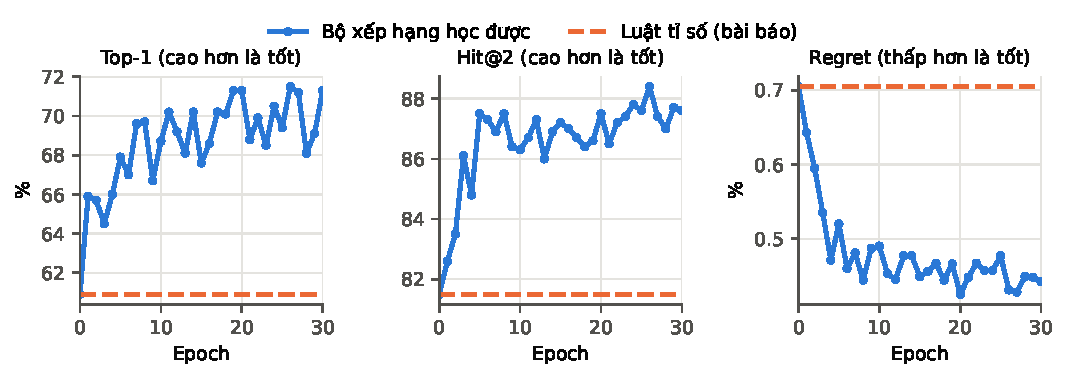
\includegraphics[width=\textwidth]{chapter4/image/ranker_training.pdf}
\caption[Chỉ số của bộ xếp hạng trên tập kiểm định qua các epoch]{Chỉ số trên tập kiểm định (10 instance chưa gặp) qua các epoch huấn luyện. Epoch 0 là mô hình chưa huấn luyện, trùng với luật tỉ số.}
\label{fig:ranker_training}
\end{figure}

\begin{table}[H]
\centering
\caption{Chất lượng xếp hạng trên tập kiểm định: luật tỉ số của E2LS so với bộ xếp hạng học được (checkpoint epoch 30).}
\label{tab:ranker_val}
\small
\begin{tabular}{lrrr}
\toprule
 & \textbf{Top-1 (\%)} & \textbf{Hit@2 (\%)} & \textbf{Regret (\%)}\\
\midrule
Luật tỉ số $R(S,i)$ & 60.9 & 81.5 & 0.705\\
Bộ xếp hạng học được & \textbf{71.3} & \textbf{87.6} & \textbf{0.442}\\
\bottomrule
\end{tabular}
\end{table}

Kết quả này cho thấy hai điều. Thứ nhất, luật tỉ số của E2LS đã khá tốt nhưng còn xa mức tối ưu: trong gần 40\% quyết định, ứng viên mà nó xếp đầu không phải là ứng viên tốt nhất, và trong 18.5\% quyết định, cả hai ứng viên được rẽ nhánh đều không tối ưu. Thứ hai, một mạng nơ-ron đồ thị nhỏ có thể học được phần lớn khoảng cách này từ dữ liệu: tỉ lệ chọn đúng tăng thêm 10.4 điểm phần trăm, tỉ lệ bỏ sót ứng viên tối ưu khỏi hai nhánh giảm từ 18.5\% xuống 12.4\%, và regret giảm 37\%. Vì tập kiểm định gồm các instance chưa gặp, mức cải thiện này phản ánh khả năng tổng quát hóa trong cùng phân phối kích thước ($m,n\le200$).

\section{Chi phí suy luận}\label{sec:cost}

Hàm xếp hạng học được phụ thuộc vào lời giải hiện tại nên phải được tính lại tại mỗi nút \addstar có nhiều hơn $a_{num}$ ứng viên. Để đo chi phí này, luận văn chạy 200 bước trên instance lớn nhất \texttt{sukp\_1000\_1000\_0.10\_0.75}, một lần với luật tỉ số và một lần với mạng (Bảng~\ref{tab:cost}).

\begin{table}[H]
\centering
\caption{Chi phí của 200 bước tìm kiếm trên \texttt{sukp\_1000\_1000\_0.10\_0.75} (CPU).}
\label{tab:cost}
\small
\begin{tabular}{lrr}
\toprule
 & \textbf{Luật tỉ số} & \textbf{Mạng}\\
\midrule
Thời gian cho 200 bước & 0.63 s & 4.03 s\\
Số lần gọi mạng & -- & 409\\
Thời gian một lần gọi mạng & -- & khoảng 9.5 ms\\
Thời gian trung bình mỗi nút \addstar (luật tỉ số) & khoảng 0.9 ms & --\\
\bottomrule
\end{tabular}
\end{table}

Mỗi lần gọi mạng tốn khoảng 9.5 mili giây, tức khoảng mười lần chi phí trung bình của một nút \addstar với luật tỉ số, và toàn bộ bước tìm kiếm chậm đi khoảng 6.4 lần. Chi phí này đến từ ba vòng truyền thông điệp trên ma trận kề dày kích thước $1000\times1000$ và từ việc gọi qua lại giữa C++ và Python. Hệ quả là ở cùng 30 giây, bộ giải dùng mạng chỉ thực hiện được khoảng một phần sáu số bước trên instance lớn. Vì vậy một hàm xếp hạng học được chỉ có lợi trong thực tế nếu chất lượng xếp hạng tốt hơn đủ để bù cho số bước bị mất. Điều này cần được kiểm chứng riêng ở chế độ cùng thời gian, và cũng là động lực cho các hướng giảm chi phí ở Chương~\ref{ch:chap5}.

\section{Đánh giá các hàm xếp hạng học được trên bộ chuẩn}\label{sec:pending}

Để đánh giá các hàm xếp hạng học được trên 60 instance chuẩn, luận văn đề xuất quy trình sau, được cài đặt trong \texttt{eval\_rankers.py} (Phụ lục~A). Mỗi cặp (instance, hàm xếp hạng) được chạy với ba seed trong hai chế độ ngân sách:
\begin{itemize}
  \item \textbf{Cùng số bước} (1000 bước tìm kiếm cục bộ): đo \emph{chất lượng xếp hạng}, vì hai bộ giải khám phá cùng số láng giềng và chỉ khác ở thứ tự rẽ nhánh của \addstar.
  \item \textbf{Cùng thời gian} (30 giây): đo \emph{giá trị thực tế}, vì thời gian suy luận của mạng được tính vào ngân sách.
\end{itemize}
Với DQN, chi phí huấn luyện trên từng instance phải được báo cáo cùng với thời gian giải. Kết quả được tổng hợp trong Bảng~\ref{tab:ranker_bench}; các ô đánh dấu đỏ sẽ được điền sau khi hoàn tất các lượt chạy.

\begin{table}[H]
\centering
\caption[Luật tỉ số so với các hàm xếp hạng học được trên bộ chuẩn]{Luật tỉ số so với các hàm xếp hạng học được trên bộ chuẩn (trung bình 3 seed). Gap: khoảng cách trung bình tới BKS. T/H/B: số instance thắng/hòa/thua so với luật tỉ số.}
\label{tab:ranker_bench}
\small
\begin{tabular}{llrrrr}
\toprule
\textbf{Ngân sách} & \textbf{Bộ} & \multicolumn{3}{c}{\textbf{Gap tới BKS (\%)}} & \textbf{T/H/B}\\
\cmidrule(lr){3-5}
 & & \textbf{Tỉ số} & \textbf{Xếp hạng} & \textbf{DQN} & \\
\midrule
1000 bước & Set I & \todo{...} & \todo{...} & \todo{...} & \todo{...}\\
1000 bước & Set II & \todo{...} & \todo{...} & \todo{...} & \todo{...}\\
30 giây & Set I & \todo{...} & \todo{...} & \todo{...} & \todo{...}\\
30 giây & Set II & \todo{...} & \todo{...} & \todo{...} & \todo{...}\\
\bottomrule
\end{tabular}
\end{table}

\section{Thảo luận}\label{sec:discussion}

\textbf{Bộ giải nền đủ mạnh để làm điểm so sánh.} Bản cài đặt C++ của E2LS với luật tỉ số đạt BKS trên 17/30 instance Set I chỉ trong 30 giây, không thua các thuật toán quần thể BABC và QL trên instance nào, và có khoảng cách trung bình 1.45\% trên Set II với ngân sách nhỏ hơn 33 lần so với E2LS gốc. Đây là một điểm so sánh chặt chẽ: một hàm xếp hạng học được phải cải thiện một bộ giải vốn đã mạnh, chứ không phải một bộ giải yếu.

\textbf{Luật tỉ số có dư địa cải thiện, và dư địa đó học được.} Trên các quyết định được gán nhãn chính xác, luật tỉ số chọn sai ứng viên tốt nhất ở gần 40\% số lần. Bộ xếp hạng học bắt chước giảm tỉ lệ này xuống còn khoảng 29\% trên instance chưa gặp, và giảm tỉ lệ bỏ sót ứng viên tối ưu khỏi hai nhánh của \addstar từ 18.5\% xuống 12.4\%. Nhờ cách tham số hóa dưới dạng hiệu chỉnh của luật tỉ số, mô hình bắt đầu từ đúng chất lượng của thuật toán gốc và chỉ thay đổi những chỗ có lợi.

\textbf{Câu hỏi còn mở là giá trị thực tế.} Có hai trở ngại giữa chất lượng xếp hạng tốt hơn và lời giải tốt hơn trên bộ chuẩn. Thứ nhất là \emph{tổng quát hóa theo kích thước}: bộ xếp hạng được huấn luyện trên $m,n\le200$ nhưng Set II có tới $m,n=1000$, và kinh nghiệm của DeepACO~\cite{Ye2023DeepACO} cho thấy mô hình học trên kích thước nhỏ vẫn có ích nhưng mất một phần lợi thế khi áp dụng cho kích thước lớn hơn nhiều. Thứ hai là \emph{chi phí suy luận}: ở cùng thời gian, bộ giải dùng mạng mất khoảng năm phần sáu số bước trên instance lớn (Mục~\ref{sec:cost}). Quy trình đánh giá ở Mục~\ref{sec:pending} được thiết kế để tách bạch hai yếu tố này: chế độ cùng số bước đo riêng chất lượng xếp hạng, còn chế độ cùng thời gian đo hiệu quả tổng thể.

\textbf{Khởi tạo lại là một điểm cắm tiềm năng khác.} Trên Set I, từ 21\% đến 44\% số bước kết thúc bằng khởi tạo lại, và thủ tục khởi tạo cũng dùng luật tỉ số. Một điểm số học được, tính một lần cho mỗi instance và dùng trong cả khởi tạo lẫn \addstar, có thể mang lại lợi ích mà gần như không tốn chi phí suy luận. Hướng này được thảo luận ở Chương~\ref{ch:chap5}.
